\subsection{Optik abbildender Systeme}
    In der geometrischen Optik (Strahlenoptik) wird das Verhalten von Licht vereinfacht modelliert. 
    \newline
    Das Verstaendnis ist wichtig, damit man weiss, wie Bild und Film auf Kamerasensoren treffen. 

    \subsubsection{Optische Systeme}
        Ein Lichtstrahl wird an Grenzflaechen wie bspw. Glas gebrochen. Dadurch entsteht eine Richtungsaenderung. Es gibt mehrere Faelle, aber fuer diesen Kurs wird nur ein Fall betrachtet: Die Strahlen treffen achsennah und parallel auf die Linse ein. Dies nennt man "paraxiale Strahlen". 
        \newline
        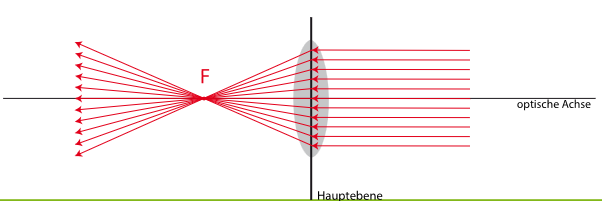
\includegraphics[width=350px]{Bilder/MINT/Paraxiale_Strahlen.png}
        \newline
        In diesem Beispiel treffen die Strahlen von rechts auf die Linse (grau) ein. Die Linse wird auch Hauptebene H genannt. Da Licht bei Glas gebrochen wird, streuen diese auf den bestimmten Punkt F zu, auf dem sie sich alle schneiden. Dieser Punkt F bestimmt, wo die Abbildung scharf ist (Fokus).
        \newline
        \textbf{Wichtig:} Nur, wenn die Strahlen von rechts eintreffen, heisst der Fokus F. Kommen sie links, ist der Fokus F'.
        \newline \newline
        Es gibt auch den Brennpunkt f - dies ist der Abstand des Fokus F von der Hauptebene H.

    \subsubsection{Abbildungsgesetze}
        Generell geht man von drei Faellen aus, was mit einem Lichtstrahl passiert. 
        SEITE 32    
\newpage